\documentclass[12pt,letterpaper]{report}

\marginparsep 0pt
\textwidth 6in
\topmargin 0pt
\headsep .5in
\textheight 9.2in
\voffset = 0pt
\hoffset = 0pt
\marginparwidth = 0pt \oddsidemargin = 0pt \sloppy

%Dimensiones de la página
\usepackage[left=2.5cm,top=3cm,right=2.5cm,bottom=2.5cm]{geometry}
%Sangría
\setlength{\parindent}{1cm}

%Numeracion
\pagenumbering{arabic}

\usepackage{templateICI}
\usepackage{amsmath,amsfonts}
\usepackage{graphicx}
\usepackage{graphics}
\usepackage[dvips]{epsfig}
\usepackage{times}
\usepackage[utf8]{inputenc}
\usepackage[dvips]{graphicx}
\usepackage[usenames]{color}
\usepackage[spanish]{babel}
\newcommand{\ie}{i.e.}
\newcommand {\out}[1]{}
\newtheorem{definicion}{Definicion}
\usepackage[dvips]{epsfig}
\usepackage{rotating}
\usepackage{multirow}
\usepackage{array}
\usepackage{longtable}
\usepackage[]{fontenc}
\usepackage{hyperref}
\usepackage{float}
\usepackage{xcolor}
\newcommand\todo[1]{\textcolor{red}{#1}}
% Esconder \todo command
%\renewcommand\todo[1]{}





\renewcommand{\shorthandsspanish}{}

\addto\captionsspanish{
\def\listtablename{Índice de tablas}
\def\tablename{Tabla}}

\sloppy

\begin{document}
\title{\textbf{Optimización de código para el prototipo de mediciones de hueso cortical}}
\author{\textbf{Claudio Antonio Araya Valenzuela}}
\principaladviser{Jean-Gabriel Minonzio}
%\coprincipaladviser{Nombre Profesor Correferente}
%\firstreader{Nombre Profesor Informante 1}

\beforepreface
\prefacesection{Resumen}

El desarrollo de alternativas mas seguras, portables y económicas a la densitometría ósea, es posible gracias a los avances en técnicas cuantitativas de ultrasonido.
La transmisión axial permite medir la porosidad y espesor cortical usando ultrasonido.
La optimización de código, permite mejorar el código existente, logrando que este se ejecute mas rápidamente.



%\newpage
%\prefacesection{Agradecimientos}
%Aqui pueden colocar sus agradecimientos.
%Si han estudiado con becas es recomendable colocar los agradecimientos a las instituciones que les otorgaron las becas.

%\afterpreface

%Aqui deben incluir el fuente de cada capitulo, sin su encabezado.
%!TEX root = templateICI.tex
%!TEX spellcheck=es_ES

\chapter{Introducci\'on}

\section{Principales contribuciones}

Los huesos son de vital importancia para la salud y la calidad de vida en general\cite{US},ya que proporcionan al cuerpo funciones estructurales y metabólicas.
Las funciones estructurales de los huesos son dar soporte para realizar las acciones mecánicas y entregar protección mecánica a distintos órganos vitales.
Metabólicamente, son encargados de producir células sanguíneas y ser la reserva de calcio mas grande del cuerpo humano
\cite{Lorincz2009}.

Los huesos se componen principalmente de dos distintos tipos de tejidos, una capa exterior compacta compuesta de hueso cortical que rodea el tejido esponjoso de hueso trabecular
\cite{Cooper2016}.

Los huesos no saludables, sin embargo, tienen un desempeño deficiente en la ejecución de sus funciones, lo que puede tener consecuencias perjudiciales como las fracturas por fragilidad
\cite{US}.
En Chile las fracturas de caderas  en adultos mayores sus costes y mortalidad equivalen a la suma de costes y mortalidad por enfermedades cardiovasculares y neoplasias
\cite{DINAMARCA-MONTECINOS2015}.

La densidad mineral osea es el marcador biológico mas usado para predecir el riesgo a fracturas, sin embargo características oseas relacionadas a la fuerza también incluyen propiedades del hueso cortical y trabecular.
Hallazgos recientes sugieren que la evaluación de riesgo de fractura también debe incluir una evaluación precisa del hueso cortical
\cite{Bala2015}.

Actualmente la empresa Azalée tiene un dispositivo de sonda multicanal para transmisión axial.
La transmisión axial es una técnica cuantitativa de ultrasonido que permite cuantificar el espesor cortical y la porosidad del hueso cortical.

La interfaz actualmente implementada despliega el espectro de ondas guiadas en casi tiempo real (con un framerate de 4Hz), siendo el tiempo de respuesta no lo suficientemente menor para el uso requerido, por lo tanto, se propone una revisión de las etapas del algoritmo usado para el análisis de los datos para encontrar secciones que se puedan optimizar.

\section{Estructura del Documento}

El documento posee la siguiente estructura. A continuación, se presenta el Marco Conceptual y el Estado del Arte, en el siguiente capitulo Definición del Problema y Análisis.

\chapter{Marco Conceptual y Estado del Arte}

En este capítulo en la sección~\ref{sc:MC} deben presentar el Marco Conceptual, así como en la sección~\ref{sc:EA} es expuesto el estado del arte. 

\section{Marco Conceptual}
\label{sc:MC}
Un marco conceptual es una sección de un texto escrito en el ámbito académico que detalla los modelos teóricos, conceptos, argumentos e ideas que se han desarrollado en relación con un tema\footnote{http://comunicacionacademica.uc.cl/images/recursos/espanol/escritura/recurso\_en\_pdf\_extenso/15\_Como\_elaborar\_un\_marco\_conceptual.pdf}. 

Si bien no existen limitaciones en esta sección, se le recomienda no sobrepasar las 5 páginas. 



\section{Estado del Arte}
\label{sc:EA}

El estado del arte es una recopilación crítica de diversos tipos de texto de un área o disciplina, el cual busca tener una visión sobre un problema específico y cómo éste se ha abordado \cite{londono2014guias}. 

Por otra parte, es importante que busque en base de datos especializadas, tales como \textit{IEEE Xplore}, \textit{Science Direct}, \textit{Springer}, \textit{ACM Digital Library}, entre otras. Un aspecto importante es que en esta sección sean discutidos entre 15 y 20 trabajos relevantes en su área de trabajo. 
%!TEX root = templateICI.tex
%!TEX spellcheck=es_ES

\chapter{Definición del Problema y Análisis}

\section{Formulación del Problema}

Actualmente la empresa Azalée cuenta con un prototipo para la medición de la porosidad y espesor oseo, este prototipo usa la técnica de transmisión axial para realizar las mediciones.
Esta es una técnica desarrollada para medir la propagación de ondas guiadas de ultrasonido en la capa cortical a lo largo del eje de huesos largos.
Los modos guiados propagados en la corteza son grabados con un arreglo de
transductor lineal de 1-MHz.
La medida de la curva de dispersión es obtenida usando una transformada de
fourier de dos dimensiones (espacio, tiempo) combinada con una descomposición
de valores singulares.
La identificación automática de parámetros es obtenida a través de la solución del problema inverso en donde las curvas de dispersión son predichas con un modelo de placa libre isotrópica transversal bidimensional.
La implementación actual de la interfaz humano-computador del prototipo tiene
tiempos de respuesta mayor al deseado.
El prototipo de medición de hueso cortical se muestra en la Figura \ref{fig:hmem}.

\begin{figure}[H]
    \centering
    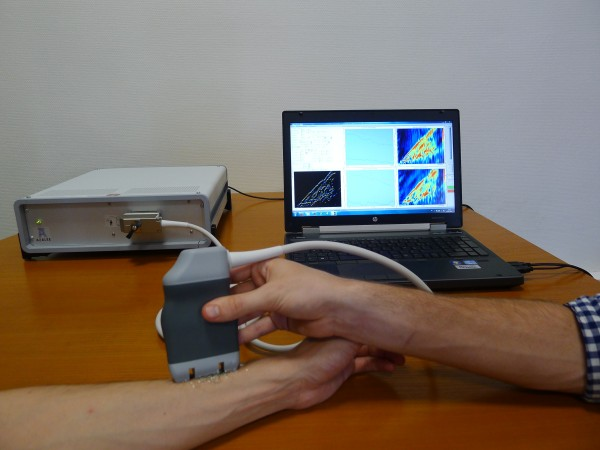
\includegraphics[width=0.75\textwidth]{imagenes/image9.jpg}
    \caption{Prototipo de Azalée.}
    \label{fig:hmem}
\end{figure}




\section{Solución Propuesta}

La solución propuesta al problema consiste en revisar las etapas del algoritmo, modificar el código para reducir complejidades temporales.
Analizar el rendimiento del software implementado para detectar los puntos problemáticos y las áreas dónde sea posible llevar a cabo una optimización del rendimiento.

\section{Objetivos}
A continuación se detallan los objetivos generales y específicos del trabajo de título

\subsection{Objetivo General}
\label{sc:OG}
Disminuir el tiempo de respuesta de la interfaz humano-computador del prototipo
de mediciones corticales de huesos, optimizando las etapas del algoritmo.


\subsection{Objetivos Específicos}
\label{ssc:OE}
\begin{enumerate}
	\item Reducir complejidades temporales del algoritmo de análisis de datos.
	\item Analizar el rendimiento del software implementado (profiling).
	\item Paralelizar código a nivel de datos y tareas.
	\item Acelerar el acceso a memoria ordenando los datos para tomar ventaja del cache del CPU.
    \item Implementar grafico de espesor/porosidad de hueso cortical mediante la resolución del problema inverso.
\end{enumerate}



\section{Metodología}
\label{sc:Met}

La metodología a usar es una cascada ad hoc al problema con una fase iterativa al final.
Esta metodología la componen las siguientes fases.
\begin{enumerate}
    \item \textbf{Aprendizaje}: Fase donde se familiarizara con los principios de la transmisión axial.
    \item \textbf{Analizar Código:} Acá el código y el algoritmo serán analizados.
    \item \textbf{Organizar Modificaciones:} Fase en la cual las modificaciones se ordenaran según las estimaciones de mejoras en el tiempo de respuesta.
    \item \textbf{Realizar modificaciones} Implementación de las modificación.
    \item \textbf{Medir} Etapas donde se prueba la modificación anteriormente realizada.
    \item Si quedan modificaciones por realizar continuar con la siguiente modificación.
\end{enumerate}


En la Figura \ref{fig:met}, se presenta un diagrama de la metodología propuesta.

\begin{figure}[H]
    \centering
    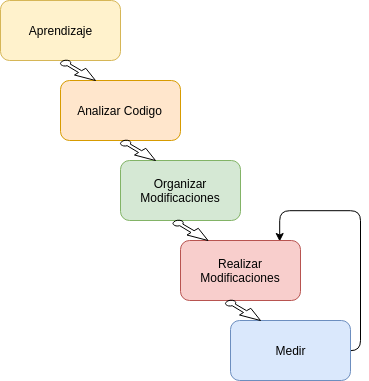
\includegraphics[width=0.75\textwidth]{imagenes/metod.png}
    \caption{Metodología a utilizar}
    \label{fig:met}
\end{figure}

\section{Especificación de Requerimientos}
\label{sc:ER}

A continuación, se detallaran los requisitos funcionales y requisitos no funcionales que el sistema de medición de hueso cortical debe cumplir.
Los requisito funcionales se entienden como una sentencia que identifica lo que el sistema debe cumplir para producir el resultado requerido deseado\cite{adams2015non}.
Los requisitos no funcionales son un requisito del software que no describe lo que el software hará, sino \emph{como} el software lo hará\cite{adams2015non}.

\subsection{Requerimientos Funcionales}
\label{ssc:RF}

En esta sección se detallan los requisitos funcionales del sistema. La sigla   \textbf{RFxx} sera usada en el documento para hacer referencia al requisito funcional.

\begin{itemize}
    \item \textbf{RF01} El sistema mostrara las graficas de espacio de Fourier de las señales recibidas por la sonda de ultrasonido.
    \item \textbf{RF02} El sistema mostrara las graficas de espesor/porosidad del hueso cortical que se este midiendo.
\end{itemize}

\subsection{Requerimientos No Funcionales}
\label{ssc:RNF}

En esta sección se detallan los requisitos no funcionales del sistema. La sigla \textbf{RNFxx} sera usada en el documento para hacer referencia al requisito no funcional.

\begin{itemize}
    \item \textbf{RNF01} El sistema mostrará las gráficas de espacio de Fourier con una frecuencia de al menos cuatro gráficos por segundo.
    \item \textbf{RNF02} El sistema mostrará las gráficas de espesor/porosidad del hueso cortical con una frecuencia de al menos cuatro gráficos por segundo.
    \item \textbf{RNF03} El sistema sera desarrollado usando el lenguaje de programación C++.
\end{itemize}

\section{Funcionalidades del Sistema}
\label{sc:FS}

\subsection{Diagramas de Casos de Uso}
\label{ssc:DCU}

El diagrama de caso de uso representa la interacción del usuario con el sistema que muestra la relación entre el usuario y los diferentes caso de uso en donde el usuario esta involucrado. En el caso del sistema de medición de hueso cortical, en la Figura \ref{fig:dcu} se muestra el único caso de uso que es realizar medición.

\begin{figure}[H]
    \centering
    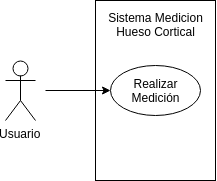
\includegraphics[width=0.75\textwidth]{imagenes/diagrama-caso-usos.png}
    \caption{Diagrama de Caso de Uso del sistema.}
    \label{fig:dcu}
\end{figure}

\subsection{Casos de Uso}
\label{ssc:CU}

% Please add the following required packages to your document preamble:
% \usepackage[normalem]{ulem}
% \useunder{\uline}{\ul}{}

En la siguiente sub-sección se presenta tabla de Caso de Uso extendido.


\begin{table}[H]
\begin{tabular}{ll}


\hline
Nombre:                     & Realizar Medición \\ \hline
Descripción:                & Permite al usuario realizar mediciones\\ &de espesor
y porosidad del hueso cortical  \\ \hline
Actores:                    & Usuario           \\ \hline
Precondiciones:             & Ninguna           \\ \hline
Requisitos No Funcionales: & RNF01,RNF02            \\ \hline
Flujo de Eventos      & 1. El usuario selecciona Realizar Medición \\
&2. Usuario alinea la sonda con el eje del largo del hueso\\
& hasta que obtiene una solución del problema inversor  \\
& 3. Finalizar medición.              \\ \hline
Post-Condiciones            & Ninguna           \\ \hline
\end{tabular}
\end{table}




\subsection{Diagramas de Secuencia}
\label{ssc:DSS}

\subsection{Diagramas de Estado}
\label{ssc:DE}


\subsection{Modelo Conceptual}
\label{ssc:MC}

%!TEX root = templateICI.tex
%!TEX spellcheck=es_ES

\chapter{Diseño}\label{ch:Diseno}

\section{Diseño Arquitectónico}\label{sc:DA}
    \subsection{Tecnologías utilizadas}\label{ssc:tech}
    En esta sección se detallaran las tecnologías a utilizar para optimizar el código del prototipo,
    para poder analizar el código (segunda etapa de la metodología a utilizar), la herramienta AutoPerf
    sera la utilizada en su ultima versión.
    Autoperf es una herramienta para crear y administrar experimentos de rendimiento, incluido el procesamiento y análisis de datos.
    Proporciona un formato simple para definir el entorno del experimento y los datos que se recopilarán, e interactúa con una variedad de herramientas de rendimiento. Junto con lo anterior, la herramienta  HPCToolkit es un conjunto integrado de herramientas para medir y analizar el rendimiento del programa en computadoras que van desde sistemas de escritorio multinúcleo a las supercomputadoras más grandes del país.
    Al utilizar un muestreo estadístico de temporizadores y contadores de rendimiento de hardware, HPCToolkit recopila mediciones precisas del trabajo, el consumo de recursos y la ineficiencia de un programa y las atribuye al contexto de llamada completo en el que se producen. HPCToolkit funciona con aplicaciones que están vinculadas estática o dinámicamente.
    Dado que HPCToolkit utiliza el muestreo, la medición tiene una sobrecarga baja (1-5\%) y se escala a grandes sistemas paralelos. Las herramientas de presentación de HPCToolkit permiten un análisis rápido de los costos de ejecución, ineficiencia y características de escalamiento de un programa tanto dentro como a través de los nodos de un sistema paralelo. HPCToolkit admite la medición y el análisis de códigos de serie, códigos de subprocesos (por ejemplo, pthreads, OpenMP), MPI y códigos paralelos híbridos (subprocesos de MPI +).

    En la etapa de Realizar Modificaciones se utilizara LIBXSMM que es una biblioteca para operaciones especializadas de matriz densa y dispersa, dirigidas a la arquitectura Intel. Los núcleos de multiplicación de matriz pequeña (SMM) se generan para Intel SSE, Intel AVX, Intel AVX2, IMCI (KNCni) para coprocesadores Intel Xeon Phi (KNC), e Intel AVX-512 tal como se encuentran en la familia de procesadores Intel Xeon Phi (KNL, KNM). ) y procesadores Intel Xeon (SKX).
    La biblioteca es compatible con el código generado de manera estática en el momento de la configuración (SMM), utiliza rutas de código optimizadas basadas en el código generado por el compilador, así como en las funciones intrínsecas, pero utiliza principalmente la especialización de código Just-In-Time (JIT) para el rendimiento independiente del compilador (multiplicaciones de matrices). , matriz de transposición / copia, funcionalidad dispersa y pequeñas circunvoluciones). LIBXSMM es adecuado para "compilar una vez e implementar en todas partes", es decir, no se necesitan indicadores de destino especiales para explotar el rendimiento disponible.
    En la tabla \ref{tab:tool} detalla las herramientas a utilizar junto con las etapas y paginas oficiales.

\begin{table}
    \begin{tabular}{|l|l|l|}
\hline
        Herramienta  & Etapa                   & Dirección Web                    \\ \hline
        HPCToolkit & Análisis de Código      & http://hpctoolkit.org/           \\
        AutoPerf   & Análisis de Código      & https://github.com/HPCL/autoperf \\
        LIBXSSM    & Realizar Modificaciones & https://github.com/hfp/libxsmm  
    \end{tabular}
    \caption{Tabla Herramientas a Utilizar.}
    \label{tab:tool}
\end{table}



    \subsection{Flujo de datos / Vista de alto nivel}\label{ssc:flow}



\section{Diseño Lógico}\label{sc:DL}
    \subsection{Diagrama de despliegue}\label{ssc:diagDesp}
    Los diagramas de despliegue (DD) se utilizan para visualizar los detalles de implementación de un sistema de software. Los diagramas incluyen más que sólo código, sino también bibliotecas separadas, un instalador, archivos de configuración y muchas otras piezas. Para que el software esté listo para ejecutarse, es necesario comprender todos los archivos y ejecutables involucrados y los entornos donde residen.

    El DD Ilustra el hardware del sistema y su software. Útil cuando se implementa una solución de software en múltiples máquinas con configuraciones únicas.

    Dos tipos especiales de dependencias: la importación de paquetes y la fusión de paquetes.

    Pueden representar los diferentes niveles de un sistema para revelar la arquitectura. Deben indicar las dependencias entre paquetes y comunicación entre estos.

    En la Figura~\ref{fig:DD}, se presenta un ejemplo de un diagrama de despliegue.

    \begin{figure}[H]
        \centering
        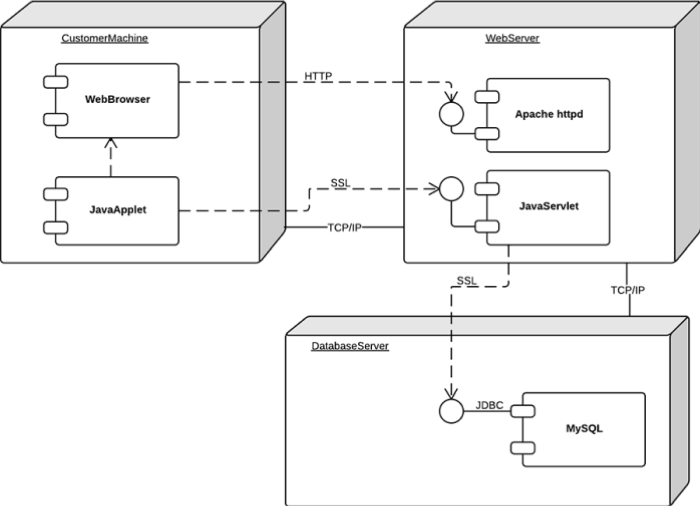
\includegraphics{imagenes/DD.png}
        \caption{Ejemplo Diagrama de Despliegue}
        \label{fig:DD}
    \end{figure}




    \subsection{Diagrama de componentes}\label{ssc:diaComp}
    En esta sección se explicara el diagrama de componentes del sistema, el componente paciente carga los datos desde el componente de Persistencia.
    El primero carga los datos en el Controlador que entrega datos a la Interfaz.
    Los datos son obtenidos desde el componente Captura Datos, que el componente Medicion se los entrega al modulo DSP.
    Finalmente, los diagramas de componentes pueden ilustrar una relación de dependencia. Una relación de dependencia ocurre cuando la interfaz provista por un componente coincide con la interfaz requerida por otro componente. La interfaz proporcionada está representada por una bola, y la interfaz requerida está representada por un \textit{socket}.

      A continuación, en la figura~\ref{fig:componentDiagram}, se presenta el diagrama de componentes para el prototipo:

        \begin{figure}[H]
        \centering
        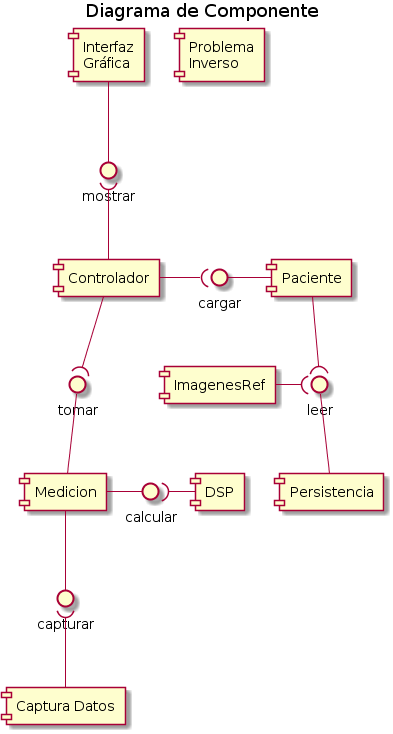
\includegraphics[width=0.7\linewidth]{imagenes/componentDiagram.png}
        \caption{Diagrama de Componentes}
        \label{fig:componentDiagram}
    \end{figure}

    Los diagramas de componentes son especialmente útiles al principio del proceso de diseño, debido a su énfasis de alto nivel. Se pueden realizar en diferentes niveles y le permiten enfocarse no sólo en los sistemas sino también en los subsistemas.


    \subsection{Diagrama de paquetes}\label{ssc:pack}

    Los diagramas de paquetes muestran los paquetes y las dependencias entre ellos. Estos diagramas pueden organizar un sistema completo en paquetes de elementos relacionados, estos podrían incluir datos, clases o incluso otros paquetes. Los diagramas de paquetes ayudan a proporcionar agrupaciones de alto nivel de un sistema para que sea fácil visualizar cómo un paquete contiene elementos relacionados, así como la forma en que los diferentes paquetes dependen entre sí.

    A continuación, en la figura~\ref{fig:packageDiagram}, se presenta un ejemplo de un diagrama de paquetes para un videojuego:

    \begin{figure}[H]
        \centering
        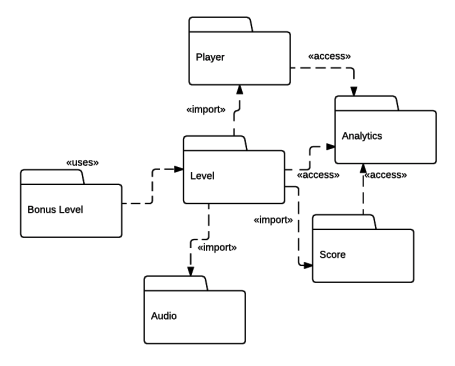
\includegraphics[width=0.7\linewidth]{imagenes/packageDiagram.png}
        \caption{Ejemplo Diagrama de Paquetes}
        \label{fig:packageDiagram}
    \end{figure}

    \subsection{Diagrama de clases}\label{ssc:clases}

El Diagrama de clase da la vista estática de una aplicación. Un diagrama de clase describe los tipos de objetos en el sistema y los diferentes tipos de relaciones que existen entre ellos. Este método de modelado se puede ejecutar con casi todos los métodos orientados a objetos.

El Diagrama de clase ofrece una descripción general de un sistema de software al mostrar clases, atributos, operaciones y sus relaciones. Este diagrama incluye el nombre de la clase, los atributos y la operación en compartimientos designados separados.

Para finalizar, el Diagrama de clase ayuda a construir el código para el desarrollo de aplicaciones de software.

Los elementos esenciales en un diagrama de clases son:

\begin{itemize}
    \item Nombre de la clase
    \item Atributos
    \item Operaciones
\end{itemize}

A continuación, en la figura~\ref{fig:classesDiagram}, se presenta un ejemplo de un diagrama de clases:
    \begin{figure}[H]
        \centering
        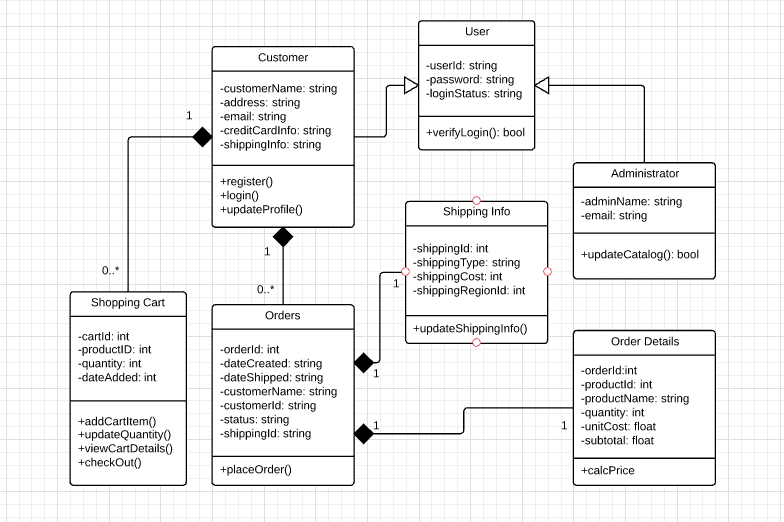
\includegraphics[width=0.7\linewidth]{imagenes/classesDiagram.png}
        \caption{Ejemplo Diagrama de Clases}
        \label{fig:classesDiagram}
    \end{figure}


\section{Diseño de Datos}\label{sc:DD}
    \subsection{Diagrama Entidad Relación}\label{ssc:ER}
    \subsection{Diagrama Relacional}\label{ssc:Rel}
    \subsection{Diccionario de Datos}\label{ssc:DD}

\section{Diseño de Interfaz}\label{sc:DI}
    \subsection{Arquitectura de la Información}\label{ssc:AA}
    \subsection{Prototipos de Interfaces Gráficas}\label{ssc:IGraph}
    %\subsection{}\label{ssc:}

\section{Diseño de Pruebas}\label{sc:DP}
    \subsection{Pruebas Unitarias}\label{ssc:UT}
    \subsection{Pruebas de Integración}\label{ssc:IT}
    \subsection{Pruebas con Usuarios}\label{ssc:PU}
    \subsection{Pruebas de Aceptación}\label{ssc:PA}

\section{Diagramas Opcionales / Complementario}\label{sc:OP}
    \subsection{Diagramas de Actividad}\label{ssc:DA}

%!TEX root = templateICI.tex
%!TEX spellcheck=es_ES

\chapter{Implementación}\label{ch:Impl}    

\section{Hardware utilizado}

El hardware utilizado para el desarrollo de esta tesis corresponde a un notebook \textbf{Lenovo B40}. Este notebook cuenta con un procesador \textbf{Intel Core i3-5005U} con una frecuencia base de 2.0 Ghz, contando con 2 núcleos. Un núcleo es un termino de hardware que describe el numero de unidades centrales de proceso independientes en un componente único de computo. La frecuencia base del procesador describe la velocidad a la que funcionan los transistores del procesador.
Este procesador cuenta con 3 niveles de cache. En el nivel 3 cuenta con 3 Megabytes de memoria, en el nivel 2 con 256 Kilobytes y el nivel 1 cuenta con 32 Kilobytes para los datos y 32 Kilobytes para las instrucciones. La CPU Cache es un área de memoria rápida ubicada en el procesador. Este procesador soporta las extensiones del conjunto de instrucciones  Intel® SSE4.1, Intel® SSE4.2, Intel® AVX2. Las Extensiones de conjunto de instrucciones son instrucciones adicionales que pueden aumentar el rendimiento cuando se realizan las mismas operaciones en múltiples objetos de datos. Estos pueden incluir SSE (Streaming SIMD Extensions) y AVX (Advanced Vector Extensions).
El notebook utilizado cuenta con 8 Gigabytes de memoria principal del tipo DDR3L. 

Todas esta características son importantes para los tiempos de ejecución del programa. La frecuencia base esta asociada a la cantidad de instrucciones que un procesador puede llevar a cabo en un tiempo determinado, la cantidad de nucleos esta ligada a la capacidad de paralelizar tareas. Las memorias cache del procesador son usadas para reducir el tiempo promedio en acceder a los datos desde la memoria principal ya que se encuentran cerca del núcleo del procesador. Las extensiones del conjunto de instrucciones nos permiten obtener paralelismo a nivel de datos.



\section{Software utilizado}
A continuación se detallaran los software utilizados para este trabajo. Se uso MATLAB que es un software para computación matemática, análisis, visualización y desarrollo de algoritmos, para el prototipo del algoritmo de transmision axial permitiendo modificar el codigo de forma mas sencilla. Se utilizo Matlab Coder para transformar el codigo en Matlab a codigo en el lenguaje de programacion C. Esta transformacion permite poder analizar el ejecutable de este codigo con HPCToolkit y asi poder identificar ineficiencias en el codigo, como subutilizacion de la cache. En este trabajo 

\section{Lenguajes de programación}
Los lenguajes utilizado fueron el lenguaje propietario de Matlab, junto con el lenguaje de programacion C. La eleccion de Matlab es por la capacidad de convertir el codigo original en codigo en C permitiendo construir binarios que se puedan analizar.  

 

\section{Estrategia de implementación}
La estrategia utilizada para implementar sera primero realizar un analisis del codigo actual y realizar un \textit{refactoring} de este. La refactorización de código es el proceso de reestructuración del código de computadora existente, sin cambiar su comportamiento externo. La refactorización está destinada a mejorar los atributos no funcionales del software. Dentro de estos cambios, primero se buscan \textit{olores de codigo}. A continuacion se listan los mas comunes.
 \begin{itemize}
 	\item \textbf{Bloaters} son código, métodos y clases que han aumentado a proporciones  que son difíciles de trabajar. Por lo general, estos olores no aparecen de inmediato, sino que se acumulan con el tiempo a medida que el programa evoluciona.
 	\item \textbf{Previene el cambio} Estos olores significan que si se necesita cambiar algo en un lugar en el código, también se tienen que hacer muchos cambios en otros lugares. El desarrollo del programa se vuelve mucho más complicado y costoso como resultado.
 	\item  \textbf{Un prescindible } es algo inútil e innecesario cuya ausencia haría que el código sea más limpio, más eficiente y más fácil de entender.
 	\item \textbf{Acopladores} los olores en este grupo contribuyen a un acoplamiento excesivo entre clases o muestran lo que sucede si el acoplamiento es reemplazado por una delegación excesiva.
 \end{itemize}

Para solucionar estos problemas se ocuparan distintas técnicas de refactoring.

\begin{itemize}
	\item \textbf{Métodos de composición} gran parte de la refactorización está dedicada a componer correctamente los métodos. En la mayoría de los casos, los métodos excesivamente largos son la raíz de todo mal. El código dentro de estos métodos ocultan la lógica de ejecución y hacen que el método sea extremadamente difícil de entender, y aún más difícil de cambiar.
	
	Las técnicas de refactorización en este grupo simplifican los métodos, eliminan la duplicación de código y allanan el camino para futuras mejoras.
	\item \textbf{Moviendo características entre objetos} muestran cómo mover de manera segura la funcionalidad entre clases, crear nuevas clases y ocultar los detalles de implementación del acceso público.
	\item\textbf{ Organizando datos} ayudan con el manejo de datos, reemplazando los primitivos con una funcionalidad de clase rica. Otro resultado importante es el desenredado de las asociaciones de clase, lo que hace que las clases sean más portátiles y reutilizables.
	\item \textbf{Simplificando Expresiones Condicionales} los condicionales tienden a complicarse cada vez más en su lógica a lo largo del tiempo.
\end{itemize}


\section{Interfaces}




%!TEX root = templateICI.tex
%!TEX spellcheck=es_ES

\chapter{Pruebas}\label{ch:testing}    

En este capítulos se realizaran pruebas para ver la concordancia entre mediciones del método fast-total con los métodos total y grad usando gráficos de Bland-Altman (agregar referencia) e histogramas con las diferencias de las mediciones de fast-total con los otros métodos. Ademas se realizaron mediciones de los tiempos de ejecución de los métodos fast-total, grad y total.

\section{Conjunto de Datos}



%!TEX root = templateICI.tex
%!TEX spellcheck=es_ES

\chapter{Resultado y Analisis de resultados}\label{ch:Impl}    

\section{Metodo Validacion}


%\appendix

%\include{appendix1}
%\include{appendix2}
%\include{appendix3}

\bibliographystyle{IEEEtran}
\bibliography{referencias,referencias/tesis}


\end{document}
